% vim: set spell spelllang=en tw=100 et sw=4 sts=4 :

\documentclass[a0paper]{tikzposter}

\usepackage{complexity}
\usepackage{wrapfig}
\usepackage{microtype}
\usepackage{gnuplot-lua-tikz}

\usepackage{lmodern}
\renewcommand*\familydefault{\sfdefault}
\usepackage[T1]{fontenc}

\title{Solving Hard Problems by Counting and Colouring Things In}
\author{Ciaran McCreesh and Patrick Prosser}
\institute{University of Glasgow, Glasgow, Scotland}
\titlegraphic{\includegraphics[keepaspectratio=true,scale=2]{UoG_keyline.eps}}

\settitle{
    \begin{tikzpicture}
        \node (T) [inner sep=0pt] {\begin{minipage}{\linewidth}
                \color{titlefgcolor}
                {\bfseries \Huge \hspace{10mm}\@title \par}
                \vspace*{1em}
                {\Large {\bfseries \hspace{10mm}\@author}, \@institute}
        \end{minipage}};

        \node at (T.east) [anchor=center, inner sep=0pt, xshift=-8cm] {\@titlegraphic};
    \end{tikzpicture}
}

% University of Glasgow standard colours

\definecolor{uofgblue}{rgb}{0, 0.321569, 0.533333}
\colorlet{uofgblue20}{uofgblue!20!white}
\colorlet{uofgblue40}{uofgblue!40!white}
\colorlet{uofgblue60}{uofgblue!60!white}
\colorlet{uofgblue80}{uofgblue!80!white}

\definecolor{uofgstone}{rgb}{0.498039, 0.454902, 0.403922}
\colorlet{uofgstone40}{uofgstone!40!white}

\definecolor{uofgtdarkgreen}{rgb}{0.380392, 0.564706, 0.501961}
\definecolor{uofgtlightgreen}{rgb}{0.615686, 0.788235, 0.729412}
\definecolor{uofgtyellow}{rgb}{0.85098, 0.827451, 0.643137}
\definecolor{uofgtorange}{rgb}{0.784314, 0.694118, 0.545098}
\definecolor{uofgtpurple}{rgb}{0.698039, 0.607843, 0.792157}
\definecolor{uofgtmauve}{rgb}{0.564706, 0.458824, 0.470588}

\definecolorstyle{UofG}{
}{
    % Background Colors
    \colorlet{backgroundcolor}{uofgstone}
    \colorlet{framecolor}{black}
    % Title Colors
    \colorlet{titlefgcolor}{white}
    \colorlet{titlebgcolor}{uofgblue}
    % Block Colors
    \colorlet{blocktitlebgcolor}{white}
    \colorlet{blocktitlefgcolor}{uofgblue}
    \colorlet{blockbodybgcolor}{white}
    \colorlet{blockbodyfgcolor}{black}
    % Innerblock Colors
    \colorlet{innerblocktitlebgcolor}{uofgblue}
    \colorlet{innerblocktitlefgcolor}{black}
    \colorlet{innerblockbodybgcolor}{uofgstone}
    \colorlet{innerblockbodyfgcolor}{black}
    % Note colors
    \colorlet{notefgcolor}{black}
    \colorlet{notebgcolor}{uofgtyellow}
    \colorlet{noteframecolor}{red}
}

\usetheme{Autumn}
\usecolorstyle{UofG}

\tikzposterlatexaffectionproofoff

\useblockstyle[bodyverticalshift=-1cm, roundedcorners=1]{Default}

\renewcommand{\Huge}{\fontsize{61.92}{77}\selectfont}

% Styles for drawings

\tikzset{edge/.style={line width=3pt, color=uofgstone}}
\tikzset{ledge/.style={line width=3pt, color=uofgstone40}}

% Colours for the graph lines

\colorlet{gp lt color 0}{uofgblue}
\colorlet{gp lt color 1}{uofgblue60}
\colorlet{gp lt color 2}{uofgblue20}
\colorlet{gp lt color 3}{uofgtorange}

\begin{document}
\maketitle

{
    \colorlet{blockbodybgcolor}{uofgtyellow}
    \colorlet{blocktitlebgcolor}{uofgtyellow}
    \block[bodyverticalshift=0cm, bodyinnersep=3mm]{}{
        \centering\begin{minipage}{0.94\textwidth}
            \textbf{Combinatorics} is a branch of mathematics devoted to counting and colouring
            things in while respecting certain rules, and \textbf{Combinatorial Optimisation} is
            about finding the ``best'' way to do this. Some important real-world problems can be
            reduced to combinatorial optimisation problems, which makes them easier to model and
            solve using computers. Our research investigates exploiting \textbf{multi-core
            parallelism} to speed up the solving process.
        \end{minipage}
    }
}

\begin{columns}
\column{0.5}

\block{Minimising Resource Usage, with Constraints}{
\begin{wrapfigure}[8]{r}{0.38\linewidth}
    \begin{center}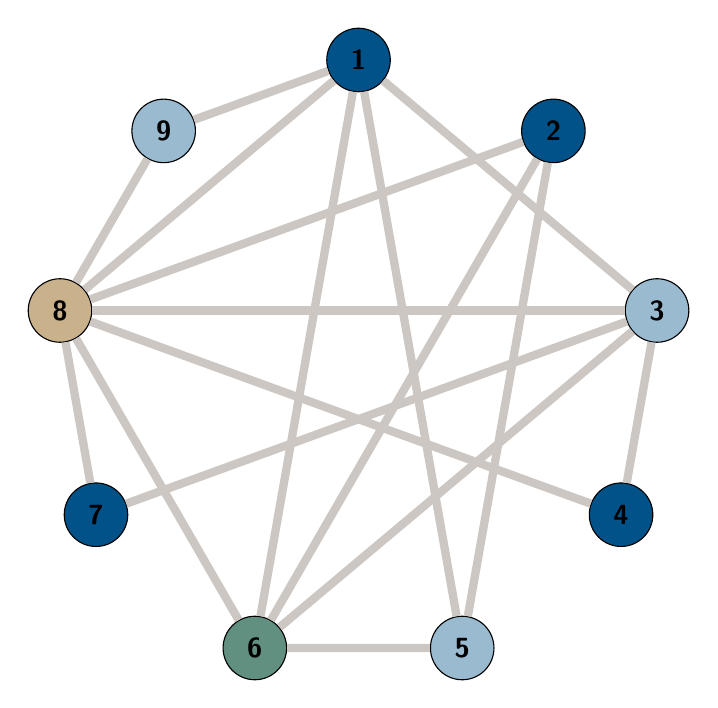
\begin{tikzpicture}[scale=1.75]%{{{
        \newcount \c
        \foreach \n in {1, ..., 9}{
            \c=\n
            \multiply\c by -40
            \advance\c by 130

            \ifthenelse{\n = 1 \OR \n = 2 \OR \n = 4 \OR \n = 7}{
                \node [draw, circle, fill=uofgblue, inner sep=5pt, font=\bfseries] (N\n) at (\the\c:2.2) {\n};
            }{
                \ifthenelse{\n = 3 \OR \n = 5 \OR \n = 4 \OR \n = 7 \OR \n = 9}{
                    \node [draw, circle, fill=uofgblue40, inner sep=5pt, font=\bfseries] (N\n) at (\the\c:2.2) {\n};
                }{
                    \ifthenelse{\n = 6}{
                        \node [draw, circle, fill=uofgtdarkgreen, inner sep=5pt, font=\bfseries] (N\n) at (\the\c:2.2) {\n};
                    }{
                        \node [draw, circle, fill=uofgtorange, inner sep=5pt, font=\bfseries] (N\n) at (\the\c:2.2) {\n};
                    }
                }
            }
        }

        \draw [ledge] (N1) -- (N5); \draw [ledge] (N1) -- (N9);
        \draw [ledge] (N2) -- (N5); \draw [ledge] (N2) -- (N6); \draw [ledge] (N2) -- (N8);
        \draw [ledge] (N3) -- (N4); \draw [ledge] (N3) -- (N7);
        \draw [ledge] (N4) -- (N8);
        \draw [ledge] (N5) -- (N6);
        \draw [ledge] (N7) -- (N8);
        \draw [ledge] (N8) -- (N9);

        \draw [ledge] (N1) -- (N3);
        \draw [ledge] (N6) -- (N8);
        \draw [ledge] (N1) -- (N6);
        \draw [ledge] (N1) -- (N8);
        \draw [ledge] (N3) -- (N6);
        \draw [ledge] (N3) -- (N8);
    \end{tikzpicture}\end{center}
\end{wrapfigure}

Suppose we need to \textbf{schedule a day's meetings}. If a person needs to attend both meeting 3
and meeting 6, then these two meetings cannot be held at the same time. We can model this as a graph
problem: we draw a circle for each meeting, and put a line between two circles if these two meetings
must occur at different times. We then want to colour in these circles, giving adjacent circles
different colours, and using as few colours as possible. By treating different colours as different
time slots, colouring in the graph gives us an optimal meeting schedule.

\medskip

We can handle richer constraints: we might have a limit on how many circles any colour can be used
in (if we only have a \textbf{limited number of meeting rooms}), or we might want each colour to be
used on the same number of circles (for a \textbf{balanced workload}).

\medskip

More generally, graph colouring tells us how to use \textbf{as few resources as possible},
respecting conflicts. Industrial uses include call centre staff allocation, scheduling jobs on
machinery, radio bandwidth allocation, and reducing the impact of vehicle maintenance.
}

\block{Finding Large, Interconnected Groups of People}{
\begin{wrapfigure}[8]{r}{0.38\linewidth}
    \begin{center}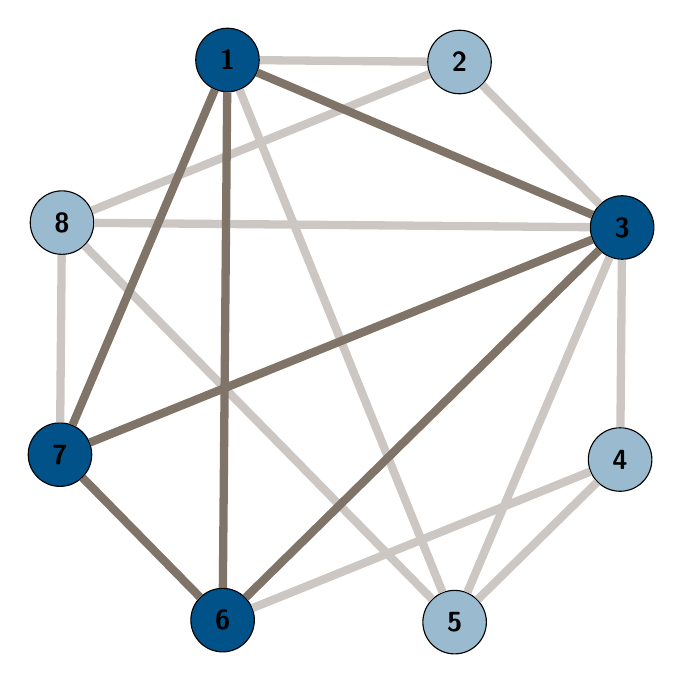
\begin{tikzpicture}[scale=1.75]%{{{
        \newcount \c
        \foreach \n in {1, ..., 8}{
            \c=\n \advance\c by -1 \multiply\c by -360 \divide\c by 8 \advance\c by 112.5
            \ifthenelse{\n = 1 \OR \n = 3 \OR \n = 6 \OR \n = 7}{
                \node[draw, circle, fill=uofgblue, inner sep=5pt, font=\bfseries] (N\n) at (\the\c:2.2) {\n};
            }{
                \node[draw, circle, fill=uofgblue40, inner sep=5pt, font=\bfseries] (N\n) at (\the\c:2.2) {\n};
            }
        }

        \draw [ledge] (N1) -- (N2);
        \draw [ledge] (N1) -- (N5);
        \draw [ledge] (N2) -- (N3);
        \draw [ledge] (N2) -- (N8);
        \draw [ledge] (N3) -- (N4);
        \draw [ledge] (N3) -- (N5);
        \draw [ledge] (N3) -- (N8);
        \draw [ledge] (N4) -- (N5);
        \draw [ledge] (N4) -- (N6);
        \draw [ledge] (N5) -- (N8);
        \draw [ledge] (N7) -- (N8);

        \draw [edge] (N1) -- (N3);
        \draw [edge] (N1) -- (N6);
        \draw [edge] (N1) -- (N7);
        \draw [edge] (N3) -- (N6);
        \draw [edge] (N3) -- (N7);
        \draw [edge] (N6) -- (N7);
    \end{tikzpicture}\end{center}
\end{wrapfigure}

    A \textbf{clique} can be thought of as a group of people, where everyone in the group knows
    everyone else in the group.  Finding cliques lets us select \textbf{as much of a resource as
    possible}, respecting compatibility rules. Clique-finding algorithms have been used to improve
    the reliability of communications and networking protocols, for social media analysis, for
    verifying electronic circuits, for targeted advertising, and for controlling flying robots.

    \medskip

\begin{wrapfigure}[10]{r}{0.38\linewidth}
    \begin{center}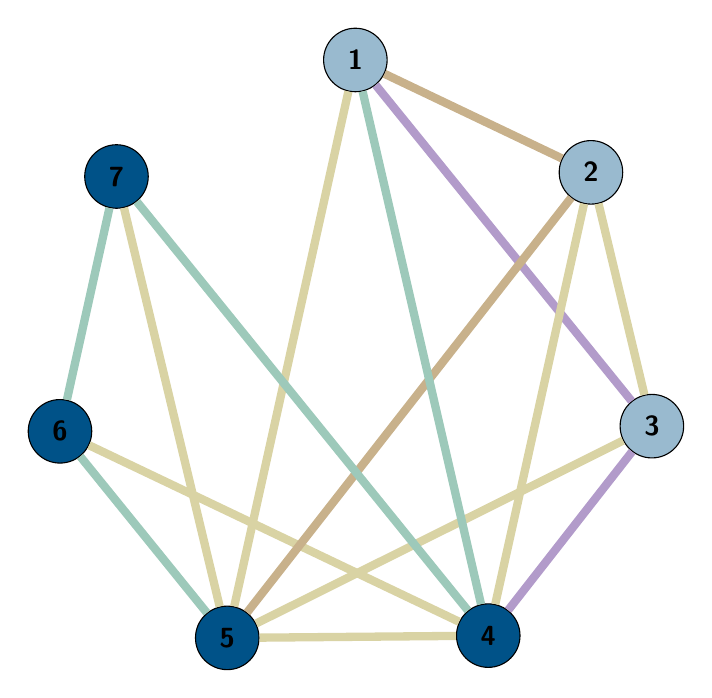
\begin{tikzpicture}[scale=1.75]%{{{
        \newcount \c
        \foreach \n in {1, ..., 7}{
            \c=\n \advance\c by -1 \multiply\c by -360 \divide\c by 7 \advance\c by 90
            \ifthenelse{\n = 1 \OR \n = 2 \OR \n = 3}{
                \node[draw, circle, fill=uofgblue40, inner sep=5pt, font=\bfseries] (N\n) at (\the\c:2.2) {\n};
            }{
                \node[draw, circle, fill=uofgblue, inner sep=5pt, font=\bfseries] (N\n) at (\the\c:2.2) {\n};
            }
        }

        \tikzstyle{l1} = [line width=3pt, color=uofgtorange];
        \tikzstyle{l2} = [line width=3pt, color=uofgtyellow];
        \tikzstyle{l3} = [line width=3pt, color=uofgtlightgreen];
        \tikzstyle{l4} = [line width=3pt, color=uofgtpurple];

        \draw [l4] (N3) -- (N4);
        \draw [l4] (N1) -- (N3);
        \draw [l2] (N1) -- (N5);
        \draw [l2] (N2) -- (N3);
        \draw [l2] (N2) -- (N4);
        \draw [l2] (N3) -- (N5);
        \draw [l2] (N4) -- (N5);
        \draw [l2] (N4) -- (N6);
        \draw [l2] (N5) -- (N7);
        \draw [l1] (N1) -- (N2);
        \draw [l1] (N2) -- (N5);
        \draw [l3] (N4) -- (N7);
        \draw [l3] (N5) -- (N6);
        \draw [l3] (N6) -- (N7);
        \draw [l3] (N1) -- (N4);
    \end{tikzpicture}\end{center}
\end{wrapfigure}

    We can add additional constraints. For example, we can label edges (representing different
    common interests, or different companies owning a network connection), and impose a budget on
    how many different labels we may use. We may also relax the adjacency requirements, requiring
    only that people be within a certain distance of each other, or that all people within a group
    all but a few other people within a group.
}

\block{Picking Out Interesting Patterns in Graphs}{
\begin{wrapfigure}[6]{r}{0.38\linewidth}
    \begin{center}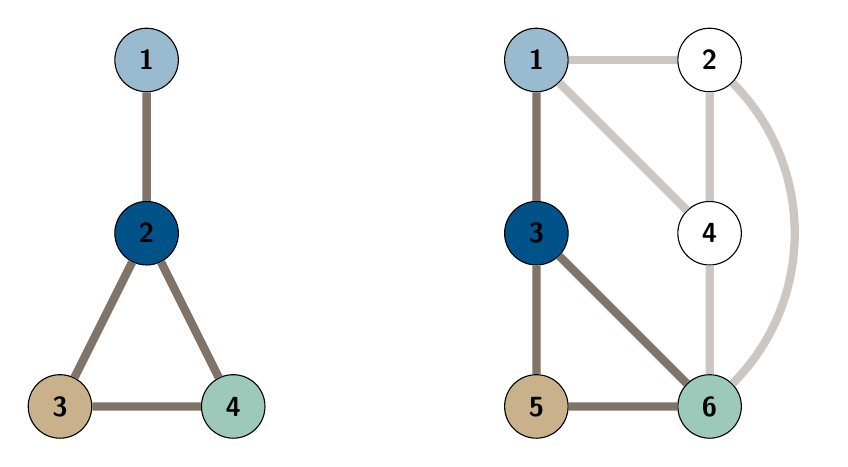
\begin{tikzpicture}[scale=1.1]%{{{
        \node[draw, circle, fill=uofgblue40, inner sep=5pt, font=\bfseries] (Na) at (1,  0) {1};
        \node[draw, circle, fill=uofgblue, inner sep=5pt, font=\bfseries] (Nb) at (1, -2) {2};
        \node[draw, circle, fill=uofgtorange, inner sep=5pt, font=\bfseries] (Nc) at (0, -4) {3};
        \node[draw, circle, fill=uofgtlightgreen, inner sep=5pt, font=\bfseries] (Nd) at (2, -4) {4};

        \draw [edge] (Na) -- (Nb);
        \draw [edge] (Nb) -- (Nc);
        \draw [edge] (Nc) -- (Nd);
        \draw [edge] (Nb) -- (Nd);

        \node[draw, circle, fill=uofgblue40, inner sep=5pt, font=\bfseries] (N1) at (5.5,  0) {1};
        \node[draw, circle, fill=white, inner sep=5pt, font=\bfseries] (N2) at (7.5,  0) {2};
        \node[draw, circle, fill=uofgblue, inner sep=5pt, font=\bfseries] (N3) at (5.5, -2) {3};
        \node[draw, circle, fill=white, inner sep=5pt, font=\bfseries] (N4) at (7.5, -2) {4};
        \node[draw, circle, fill=uofgtorange, inner sep=5pt, font=\bfseries] (N5) at (5.5, -4) {5};
        \node[draw, circle, fill=uofgtlightgreen, inner sep=5pt, font=\bfseries] (N6) at (7.5, -4) {6};

        \draw [ledge] (N1) -- (N2);
        \draw [edge] (N1) -- (N3);
        \draw [ledge] (N1) -- (N4);
        \draw [ledge] (N2) -- (N4);
        \draw [edge] (N3) -- (N5);
        \draw [edge] (N3) -- (N6);
        \draw [ledge] (N4) -- (N6);
        \draw [edge] (N5) -- (N6);
        \draw [ledge] (N2) to [in=45, out=315] (N6);

    \end{tikzpicture}\end{center}
\end{wrapfigure}

    The \textbf{subgraph isomorphism} problem is to find a small ``pattern'' graph in a big
    ``target'' graph. This is useful in drug design, in fraud detection, and in fault diagnosis.

    \vspace{1em}

    The \textbf{maximum common subgraph} problem finds the largest subgraph common to two bigger
    graphs. This in turn allows us to see how similar two graphs are. This is useful in computer
    vision and in biochemistry.
}


\column{0.5}

\block{More Flexibility via Constraint Programming}{
    These techniques can be used for \emph{any} system where we have some variables, and some
    constraints between those variables, and we wish to instantiate the variables whilst respecting
    all the constraints. This is called \textbf{constraint programming}.  Large-scale industrial
    successes for constraint programming include:

\begin{itemize}
    \item Timetabling a national railway system.
    \item Improving vehicle delivery routes.
    \item Reducing production costs in lumber processing.
    \item Producing greener and more energy-efficient data centres.
    \item Scheduling the Rosetta / Philae mission operations.
    \item Automatic test generation.
    \item Reducing waste and improving quality in wine blending.
    \item Reducing the cost of an invasion.
    \item Scheduling airport gate and crew allocations.
    \item Organising sporting seasons for optimal TV coverage.
\end{itemize}

\vspace{1em}

\begin{center}
    \includegraphics*[keepaspectratio=true,height=8.5cm]{train.jpg}
    \hfill
    \includegraphics*[keepaspectratio=true,height=8.5cm]{comet.jpg}
    \hfill
    \includegraphics*[keepaspectratio=true,height=8.5cm]{airport.jpg}
\end{center}

\vspace{1em}

Constraint programming toolkits are also better than you at solving Sudoku puzzles: groups of
variables which must be ``all different'' form the core of many interesting applications, and
network flow algorithms give powerful, efficient inference for these constraints.

\vspace{1em}

\begin{center}\begin{tikzpicture}
\newcounter{row}
\newcounter{col}

\newcommand\setrow[9]{
    \setcounter{col}{1}
    \foreach \n in {#1, #2, #3, #4, #5, #6, #7, #8, #9} {
        \newcount \x
        \newcount \y
        \x=\value{col}
        \advance \x by -1
        \multiply \x by 3
        \y=9
        \advance \y by -\value{row}
        \multiply \y by 3
        \node[anchor=center] at ($(\x + 1.5, \y + 1.5)$) {\huge\n};
        \stepcounter{col}
    }
    \stepcounter{row}
}

\draw[very thick, scale=3, color=uofgstone40] (0, 0) grid (9, 9);
\draw[very thick, scale=9, color=uofgstone] (0, 0) grid (3, 3);

\setcounter{row}{1}

\setrow { }{ }{ } { }{ }{ } {5}{4}{ }
\setrow { }{ }{ } { }{ }{3} {8}{ }{ }
\setrow { }{ }{8} {7}{1}{ } { }{2}{ }

\setrow { }{1}{7} {4}{ }{ } { }{8}{ }
\setrow {4}{ }{ } { }{ }{ } { }{ }{2}
\setrow { }{ }{ } { }{ }{ } { }{3}{1}
:
\setrow {2}{ }{ } {1}{ }{ } { }{6}{ }
\setrow {7}{ }{ } { }{ }{8} { }{ }{ }
\setrow { }{6}{3} { }{ }{7} { }{ }{ }

\end{tikzpicture}\end{center}

\vspace{1em}
}

\end{columns}

\block{Research Area: Practical Techniques for Solving Hard Problems in Parallel}{
\begin{wrapfigure}[15]{r}{0.38\linewidth}
    \begin{center}\begin{tikzpicture}
        \input{gen-graph-speedup}
    \end{tikzpicture}\end{center}
\end{wrapfigure}

    Combinatorial optimization is, in general, a \textbf{hard problem} (like the famous
    \textbf{travelling salesman problem}): every additional variable we add in can double the
    difficulty of finding a solution, so the time taken to solve a problem grows exponentially. In
    practice we can usually avoid this worst case, but solving these problems still takes longer
    than we would like.

    \medskip

    Modern processors have at least two, and sometimes as many as fifteen, processing cores. We
    might hope that we could use these cores to make our programs \textbf{run faster},
    or at least to allow us to \textbf{solve larger problems} in the time we have.

    \medskip

    In general, we do this by splitting problems up into evenly sized, independent pieces of work,
    which may be evaluated in parallel. However, combinatorial optimisation
    problems tend to be \textbf{highly irregular} (cannot be split into evenly sized pieces) and
    require \textbf{speculative parallelism} (the pieces have dependencies upon each other, and we
    must guess what the answer might be allow parallel evaluation).

    \medskip

    Despite this, results can be favourable. Our approach uses parallelism to explicitly
    \textbf{introduce diversity} into a search process to offset the weakest choices made by
    heuristics, so our parallel workers are reducing our commitment to potentially costly early
    mistakes. This is combined with late rebalancing, to give good work balance with low overheads
    and good scalability.
}

{
    \colorlet{blockbodybgcolor}{uofgstone}
    \colorlet{blocktitlebgcolor}{uofgstone}
    \block[bodyverticalshift=-0.5cm]{}{
        \texttt{c.mccreesh.1@research.gla.ac.uk}

        \flushleft\small
        Photos: Wikimedia ``VIRM6.jpg'' (Maurits90) (cropped), Wikimedia ``Rosetta and Philae at comet
        (11206660686).jpg'' (ESA-C. Carreau/ATG medialab), Wikimedia
        ``A\_bird's\_eye\_view\_of\_Hong\_Kong\_International\_Airport.JPG'' (Wylkie Chan).
    }
}

\end{document}

